\documentclass[12pt]{article}

%%novalidate

\usepackage{tikz}
\usepackage{calc}
\usepackage{booktabs}
%\usepackage{hyperref}
\usepackage[utf8]{inputenc}
\usepackage[T1]{fontenc}
\usepackage{graphicx}
\usepackage{xcolor}
\usepackage{kotex}

%소스코드 추가를 위한 패키지
\usepackage{listings}

\definecolor{codegreen}{rgb}{0,0.6,0}
\definecolor{codegray}{rgb}{0.5,0.5,0.5}
\definecolor{codepurple}{rgb}{0.58,0,0.82}
\definecolor{backcolour}{rgb}{0.95,0.95,0.92}

\lstdefinestyle{mystyle}{
	backgroundcolor=\color{backcolour},   
	commentstyle=\color{codegreen},
	keywordstyle=\color{magenta},
	numberstyle=\tiny\color{codegray},
	stringstyle=\color{codepurple},
	basicstyle=\footnotesize,
	breakatwhitespace=false,         
	breaklines=true,                 
	captionpos=b,                    
	keepspaces=true,                 
	numbers=left,                    
	numbersep=5pt,                  
	showspaces=false,                
	showstringspaces=false,
	showtabs=false,                  
	tabsize=2
}

\lstset{style=mystyle}

% colors
\definecolor{color1}{HTML}{000060}
%\definecolor{color1}{HTML}{8C260F}
\definecolor{color2}{HTML}{333333}


% fonts
\usepackage{fontspec}
\defaultfontfeatures{Mapping=tex-text}
\setmainfont
[BoldFont=HDHarmony_B.ttf,
ItalicFont=Lato-Italic.ttf,
BoldItalicFont=Lato-BoldItalic.ttf]
%{Lato-Regular.ttf}
{HDHarmony.ttf}
\newfontfamily\headingfont[ItalicFont=Lato-BlackItalic.ttf]{HDHarmony_B.ttf}
%%%

\usepackage{geometry}
\geometry{a4paper,
hmargin=20mm,vmargin=20mm,
head=0ex,foot=3ex}

\linespread{1.3}

\usepackage[hang]{caption}
\DeclareCaptionFormat{upper}{#1#2\uppercase{#3}\par}
\captionsetup{labelfont={bf,color=color2},textfont={normalsize,color=color2},format = upper,figurename=FIGURE,tablename=TABLE}

%%% fancy sections
\usepackage{titlesec}
%\titleformat{\chapter}{\headingfont\LARGE\bfseries\scshape\color{color1}}{\thechapter}{1em}{}[\titlerule]
%\titleformat{\section}{\color{color1}\headingfont\Large\bfseries\uppercase}{\thesection}{1em}{}[\titlerule]
%\titleformat{\subsection}{\color{color1}\headingfont\large\bfseries\uppercase}{\thesubsection}{1em}{}
%\titleformat{\subsubsection}{\color{color1}\headingfont\bfseries\uppercase}{\thesubsubsection}{1em}{}
%Title의 재목이 항상 대문자로 표시되기 때문에, \uppercase 문을 삭제함
\titleformat{\section}{\color{color1}\headingfont\Large\bfseries}{\thesection}{1em}{}[\titlerule]
\titleformat{\subsection}{\color{color1}\headingfont\large\bfseries}{\thesubsection}{1em}{}
\titleformat{\subsubsection}{\color{color1}\headingfont\bfseries}{\thesubsubsection}{1em}{}
%%%

% head and foot
\usepackage{fancyhdr}
\pagestyle{fancy}
\lhead{}
\chead{}
\makeatletter
\rhead{\color{color2}\@date}
\makeatother
\newlength{\myheight}
\lfoot{
\settoheight{\myheight}{\thepage}
\raisebox{-2ex-0.5\myheight}{
\includegraphics[height=4ex]{HMC_logo}}
}
\cfoot{\color{color2}ccOS Document}
\rfoot{\color{color2}\thepage}
\renewcommand\headrulewidth{0pt}
\renewcommand\footrulewidth{0pt}

%%% picture on cover page
\usepackage{eso-pic}
\newcommand\BackgroundPic{%
\put(0,0){%
\parbox[b][\paperheight]{\paperwidth}{%
\vfill
\centering
% Cover page의 그림은 일단 삭제
%
\includegraphics[width=\paperwidth,height=\paperheight,%
%keepaspectratio]{cover}%
\vfill
}}}
%%%
% custom titlepage
\makeatletter
\renewcommand{\maketitle}{
\thispagestyle{empty}
\AddToShipoutPicture*{\BackgroundPic}
\ClearShipoutPicture
%
\phantom{a}
\vfill
\phantom{a}\hfill
%    \color{black}\headingfont\LARGE\@title\\[1em]
%    \color{black}\headingfont\Large\@author\\[2em]
\begin{tabular}[c]{@{}p{0.7\textwidth}@{}}
%      \color{white}\headingfont\LARGE\@title\\[1em]
 %     \color{white}\headingfont\Large\@author\\[2em]
     \color{black}\headingfont\LARGE\@title\\[1em]
    \color{black}\headingfont\Large\@author\\[2em]
\end{tabular}
%
\clearpage
}
\makeatother
%%%


%%% fancy boxes
\usepackage{tcolorbox}
\usepackage{wrapfig}
\def\fullboxbegin{
\bigskip
\begin{tcolorbox}[colback=color1,colframe=color1,coltext=white,arc=0mm,boxrule=0pt]
}
\def\fullboxend{\end{tcolorbox}\medskip}
%
\def\leftboxbegin{
\begin{wrapfigure}{l}{0.5\textwidth}
\begin{tcolorbox}[colback=color1,colframe=color1,coltext=white,arc=0mm,boxrule=0pt]
}
\def\leftboxend{
\end{tcolorbox}
\end{wrapfigure}
}
%
\def\rightboxbegin{
\begin{wrapfigure}{r}{0.5\textwidth}
\begin{tcolorbox}[colback=color1,colframe=color1,coltext=white,arc=0mm,boxrule=0pt]
}
\def\rightboxend{
\end{tcolorbox}
\end{wrapfigure}
}
%
\newcounter{frames}
\def\frameboxbegin#1{
\bigskip
\refstepcounter{frames}
\begin{tcolorbox}[colback=white,colframe=color1,arc=0mm,title={\MakeUppercase{\textbf{Frame \arabic{frames}}: #1}}]
}
\def\frameboxend{
\end{tcolorbox}
}

\newcounter{subsubsubsection}[subsubsection]
\def\subsubsubsectionmark#1{}
\def\thesubsubsubsection {\thesubsubsection 
	.\arabic{subsubsubsection}}
\def\subsubsubsection{\@startsection
	{subsubsubsection}{4}{\z@} {-3.25ex plus -1
		ex minus -.2ex}{1.5ex plus .2ex}{\normalsize\bf}}
\def\l@subsubsubsection{\@dottedtocline{4}{4.8em}
	{4.2em}}


%\newcommand{cmd}[args][default]{def}
%%%

\titleformat{\paragraph}[hang]{\normalfont\normalsize\bfseries}{\theparagraph}{1em}{}
\titlespacing*{\paragraph}{0pt}{3.25ex plus 1ex minus .2ex}{0.5em}

\titleformat{\subparagraph}
{\normalfont\normalsize\bfseries}{\thesubparagraph}{1em}{}
\titlespacing*{\subparagraph}{\parindent}{3.25ex plus 1ex minus .2ex}{.75ex plus .1ex}

\usepackage{indentfirst}
\setlength{\parindent}{0.5cm}% too much in my eyes delete this
% line and use the default ...


%%%%%%%%%%%%%%%%%%%%%%%%
% Section 넘버링 depth 설정
\setcounter{secnumdepth}{5}
\setcounter{tocdepth}5


%%%%%%%%%%%%%%%
% Title Page
\title{ccOS Lifecycle}
\author{Infotainment Software Development Team \newline Hyundai Motor Company \newline }
\date{\today}
%%%%%%%%%%%%%%%

\begin{document}
	\maketitle
	
	\tableofcontents
	
	%%%%%%%%%%%%%%%%%%%%%%%%%%%%%%%%%%%%%%%%%%%%%%%%%%
	% 본문의 시작 
	%%%%%%%%%%%%%%%%%%%%%%%%%%%%%%%%%%%%%%%%%%%%%%%%%%
	\clearpage
	\section{서론}
	
	편향(bias)는 뉴런이 얼마나 쉽게 활성화 되는지를 제어한다.
	가중치는 각 신호의 영향력을 의미한다.
	
	\subsection{목적}
	
	\begin{figure}[!h] %신경망 예시 그림
		\centering
		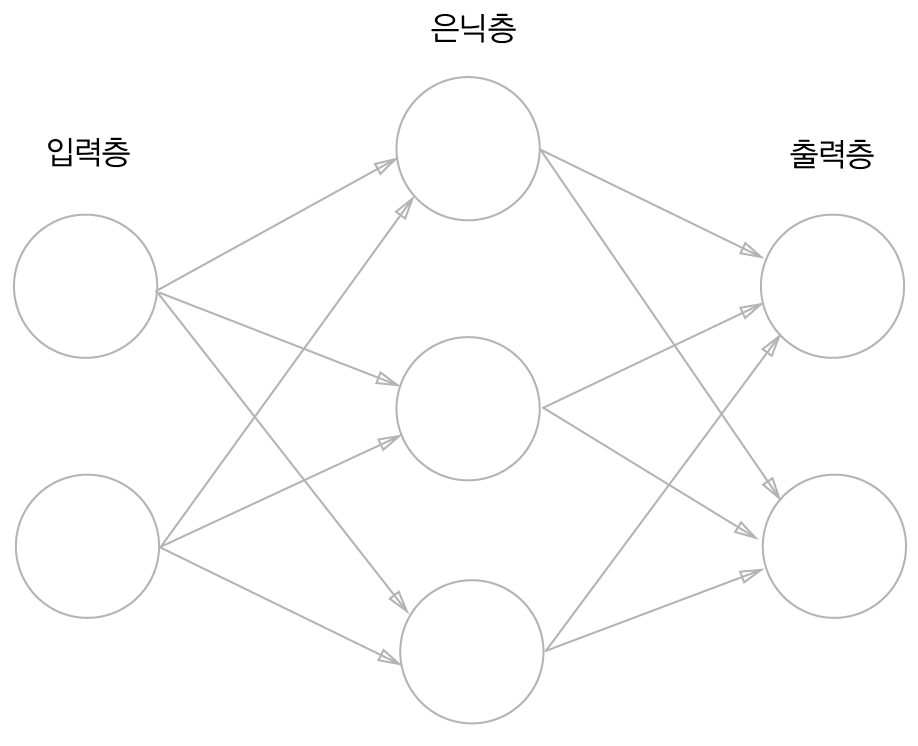
\includegraphics[width=0.8\textwidth]{fig/fig-3-1.png}
		\caption{신경망의 예}
	\end{figure}
	
	
	Perceptron은 복잡한 함수도 표현이 가능하다. 심지어 다층 퍼셉트론은 컴퓨터도 표현 가능하다.
	하지만, 퍼셉트론의 가중치를 설정하는 것은 여전히 사람에 의해서만 가능하다.
	
	신경망은 데이터로 부터 퍼셉트론의 가중치 설정을 자동으로 한다.
	
	\clearpage
	\section{신경망}
	입력층, 은닉층, 출력층 으로 구성
	활성화 함수 - 입력 신호의 총합을 출력 신호로 변환
	
	활성화 함수를 계단 함수에서 다른 함수로 변경하는 것이 신경망의 세계로 나아가는 열쇠이다.
	
	% $f(x)=\frac{1}{1+e^{-x}}$
	\[ f(x)=\frac{1}{1+\exp^(-x)}	\]
	
	신경망의 활성화 함수는 비선형 함수를 사용해야 한다. 여기서 비선형이란 하나의 직선으로 표현할 수 없는 함수를 의미한다.
	비선형 함수를 사용하는 이유는 선형 함수를 사용할 경우 신경망 층을 깊게 하면 의미가 사라지기 때문이다.
	
	신경망은 분류와 회귀에 이용할 수 있다. 이는 출력층의 활성화 함수의 선택을 결정 짓는 요인이 된다. 회귀에는 항등함수를 사용하고 분류에는 소프트맥스함수를 사용한다.
	
	\subsection{소프트맥스 함수의 특징}
	소프트맥스 함수의 출력은 0과 1.0사이의 실수이며, 함수 출력 총합은 1이다.
	이러한 성질을 이용하면 소프트맥스 함수의 출력을 확률로 생각할 수 있다.
	\[ f(v) = \frac{\exp(a_{k})} {\sum_{i=1}^{n}  {\exp(a_{i})}} \]
	
	소프트맥스 함수는 단조 증가 함수이기 때문에 소프트맥스 함수를 활성함수로 적용해도 각 원소의 대소 관계는 변화가 없다. 따라서, 신경망을 이용하여 분류를 할때 출력층의 소프트맥스 함수를 생략할 수 있다.
	
	\subsection{궁금한점}
	하지만, 분류에 소프트맥스 함수를 생략 할 수 있다면 결국 항등 함수와 무엇이 다른가?
	\clearpage
	
\section{신경망 학습}
학습이한 데이터로 부터 가중치 매개 변수의 최적값을 자동으로 획득한다.
그렇다면 어떻게 매개 변수가 최적값인지를 판단할 수 있을까?
즉, 매개 변수에 대한 평가 방법이 필요하며 이러한 역할은 손실 함수가 수행한다.
손실 함수가 매개 변수 성능에 대한 결과를 정량적인 수치로 나타낸다면, 
신경망의 학습 목표는 손실 함수의 값을 작게 만드는 매개 변수를 찾는 것이다.

어떻게 하면 손실함수의 값을 작게 만들 수 있을까?
이는 손실 함수와 매개 변수와의 관계를 다시 생각해 보게 한다.
매개 변수가 손실 함수에 미치는 영향을 분석하여 각 매개 변수가 음(-)이나 양(+)의 방향과 그 정도를 통해
손실 함수를 가능한한 최소화하는 값을 찾을 수 있고 이러한 방법을 경사법이라 한다.


딥러닝은 종단간 기계학습(end-to-end machine learning)이라고도 한다. 데이터(입력)에서 목표한 결과(출력)을 사람의 개입없이 얻는다는 의미.

\subsection{손실함수}

손실함수는 평균 제곱 오차(mean squared error, MSE)와 교차 엔트로피 오차(cross entropy error, CEE) 둘이 자주 사용된다.
\subsubsection{평균 제곱 오차}
평균 제곱 오차의 식은 다음과 같다.
\[ E = \frac{1}{2} \sum_{k}(y_{k} - t_{k})^2  \]

이때 궁금한 점은 평균임에도 불구하고 왜 n이 아닌 2로 나누는 것인가? 이는 y값과 t값이 갖는 범위를 생각해 보면 이해할 수 있다. 먼저 y는 소프트맥스함수 값이므로 $y_{k}$ 총 합은 항상 1이다.
$t_{k}$는 원-핫 인코딩으로 표기 했기 때문에 정답에 해당하는 값만 1이고 나머지는 0이다. 따라서 $t_{k}$의 총합 또한 항상 1이다. 따라서 이들의 평균을 구하기 위해서는 N이 아닌 2로 나누어야 한다.

평균 제곱 오차의 값이 작을 수록 정답에 가깝고 값이 클 수록 정답이 아님을 의미한다.
	\subsubsection{교차 엔트로피}
	교차 엔트로피는 

\subsection{ 편미분}
\begin{lstlisting}[language=Python, caption={Python으로 구현한 편미분 함수},label=gradient-function]
def numerical_gradient(f, x):
	h = 1e-4
	grad = np.zeros_like(x)

	for idx in range(x.size):
		tmp_val = x[idx]
		x[idx] = tmp_val + h
		fxh1 = f(x)

		x[idx] = tmp_val - h
		fxh2 = f(x)

		grad[idx] = (fxh1 - fxh2) / (2*h)
		x[idx] = tmp_val

	return grad
\end{lstlisting}

Listing \ref{gradient-function}은 편미분을 구하는 python함수이다. Line1의 함수의 선언에서와 같이 편미분을 구하는 numerical\_gradient함수는 인자로 편미분을 구하고자 하는 함수 f와 그때의 좌표를 np.array형인 x로 받는다.

\end{document}          
